%! Author = stephane
%! Date = 18.02.22

% Preamble
\documentclass[10pt,a4paper]{report}
% Gestion du titre
\author{Stéphane Bressani}
\title{Recettes de cuisines}

% Packages
\usepackage[utf8]{inputenc} % Encodage d'entrée
\usepackage[frenchb]{babel} % Langage
\usepackage[T1]{fontenc} % Encodage de sortie
\usepackage{graphicx} % Extension pour les images
\usepackage[left=2cm, right=2cm, top=2cm, bottom=2cm]{geometry} % marges

\usepackage{blindtext}
\usepackage{multicol}
\setlength{\columnsep}{15pt}
\setlength{\columnseprule}{1pt}


% Document
\begin{document}
    % Affichage du titre
    \maketitle
    % Affichage de la table des matières
    \tableofcontents

    \chapter{Repas chaud}
    % Section
    \section{Omelette espagnole}

    \begin{multicols}{2}
        \parbox[1cm]{\textwidth}{
            \begin{description}
                \item \textit{3 cuillère à soupe d'huile d'olive}
                \item \textit{1 à 2 oignons hachés}
                \item \textit{2 gousses d'ail écrasées}
                \item \textit{1 poivron rouge évidé et haché}
                \item \textit{4 oeufs}
                \item \textit{sel et poivre}
                \item \textit{2 grosses pommes de terre cuites et émincées}
                \item \textit{2 cuillères à soupe de persil haché}
            \end{description}
        }
        \columnbreak

        Faites chauffer 2 cuillère à soupe d'huile dans une poêle de 24 cm, ajoutez et faites revenir les oignons. Ajouter l'ail, le poivron et laissez cuire 10 minutes.
        \newline

        Battez les oeufs dans une jatte avec le sel, le poivre, puis ajoutez-leur les pommes de terre, le persil et le mélange précédent.
        \newline

        Faites chauffer le reste d'huile dans la poêle, versez le mélange et laissez cuire 5 minutes, en secouant la poêle.
        \newline
        \newline
        \textbf{Pour 4 personnes}
    \end{multicols}

    \newpage
    % Section
    \section{Curry de haricots}

    \begin{multicols}{2}
        \parbox[1cm]{\textwidth}{
            \begin{description}
                \item \textit{500g de haricots noirs ayabt trempé une nuit}
                \item \textit{sel}
                \item \textit{3 cuillères à café de cumin moulu}
                \item \textit{1 cuillère à café de garam massala}
                \item \textit{1 pincée de Cayenne}
                \item \textit{1 cm de gingembre haché}
                \item \textit{4 gousses d'ail pilées}
                \item \textit{400g de tomates}
                \item \textit{3 branches de céleri}
                \item \textit{1 cuillère a café de cardamome}
                \item \textit{1 cuillère à soupe de corandre hachée}
            \end{description}
        }
        \columnbreak

        Égouttez les haricots, mettez-les dans une casserole, couvrez d'eau froide, portez à ébullition et laissez bourillir 10 minutes, puis couvrez et laissez frémir 1h30, en salant à la fin. Mettez de côté 30 cl de liquide de cuisson.
        \newline

        Faites chauffer l'huile dans une casserole, ajoutez et faites revenir les oignons. Ajoutez le cumin, le garam massala, le Cayenne, le gingembre, l'ail et tournez 1 minute. Ajoutez le liquide de cuissons, les haricots, les tomates écrasées, le céleri haché, les grains de cardamome, salez, couvrez et laissez frémir 45 minutes. Ajoutez la coriandre fraîche. Servez avec du riz.
        \newline
        \newline
        \centerline{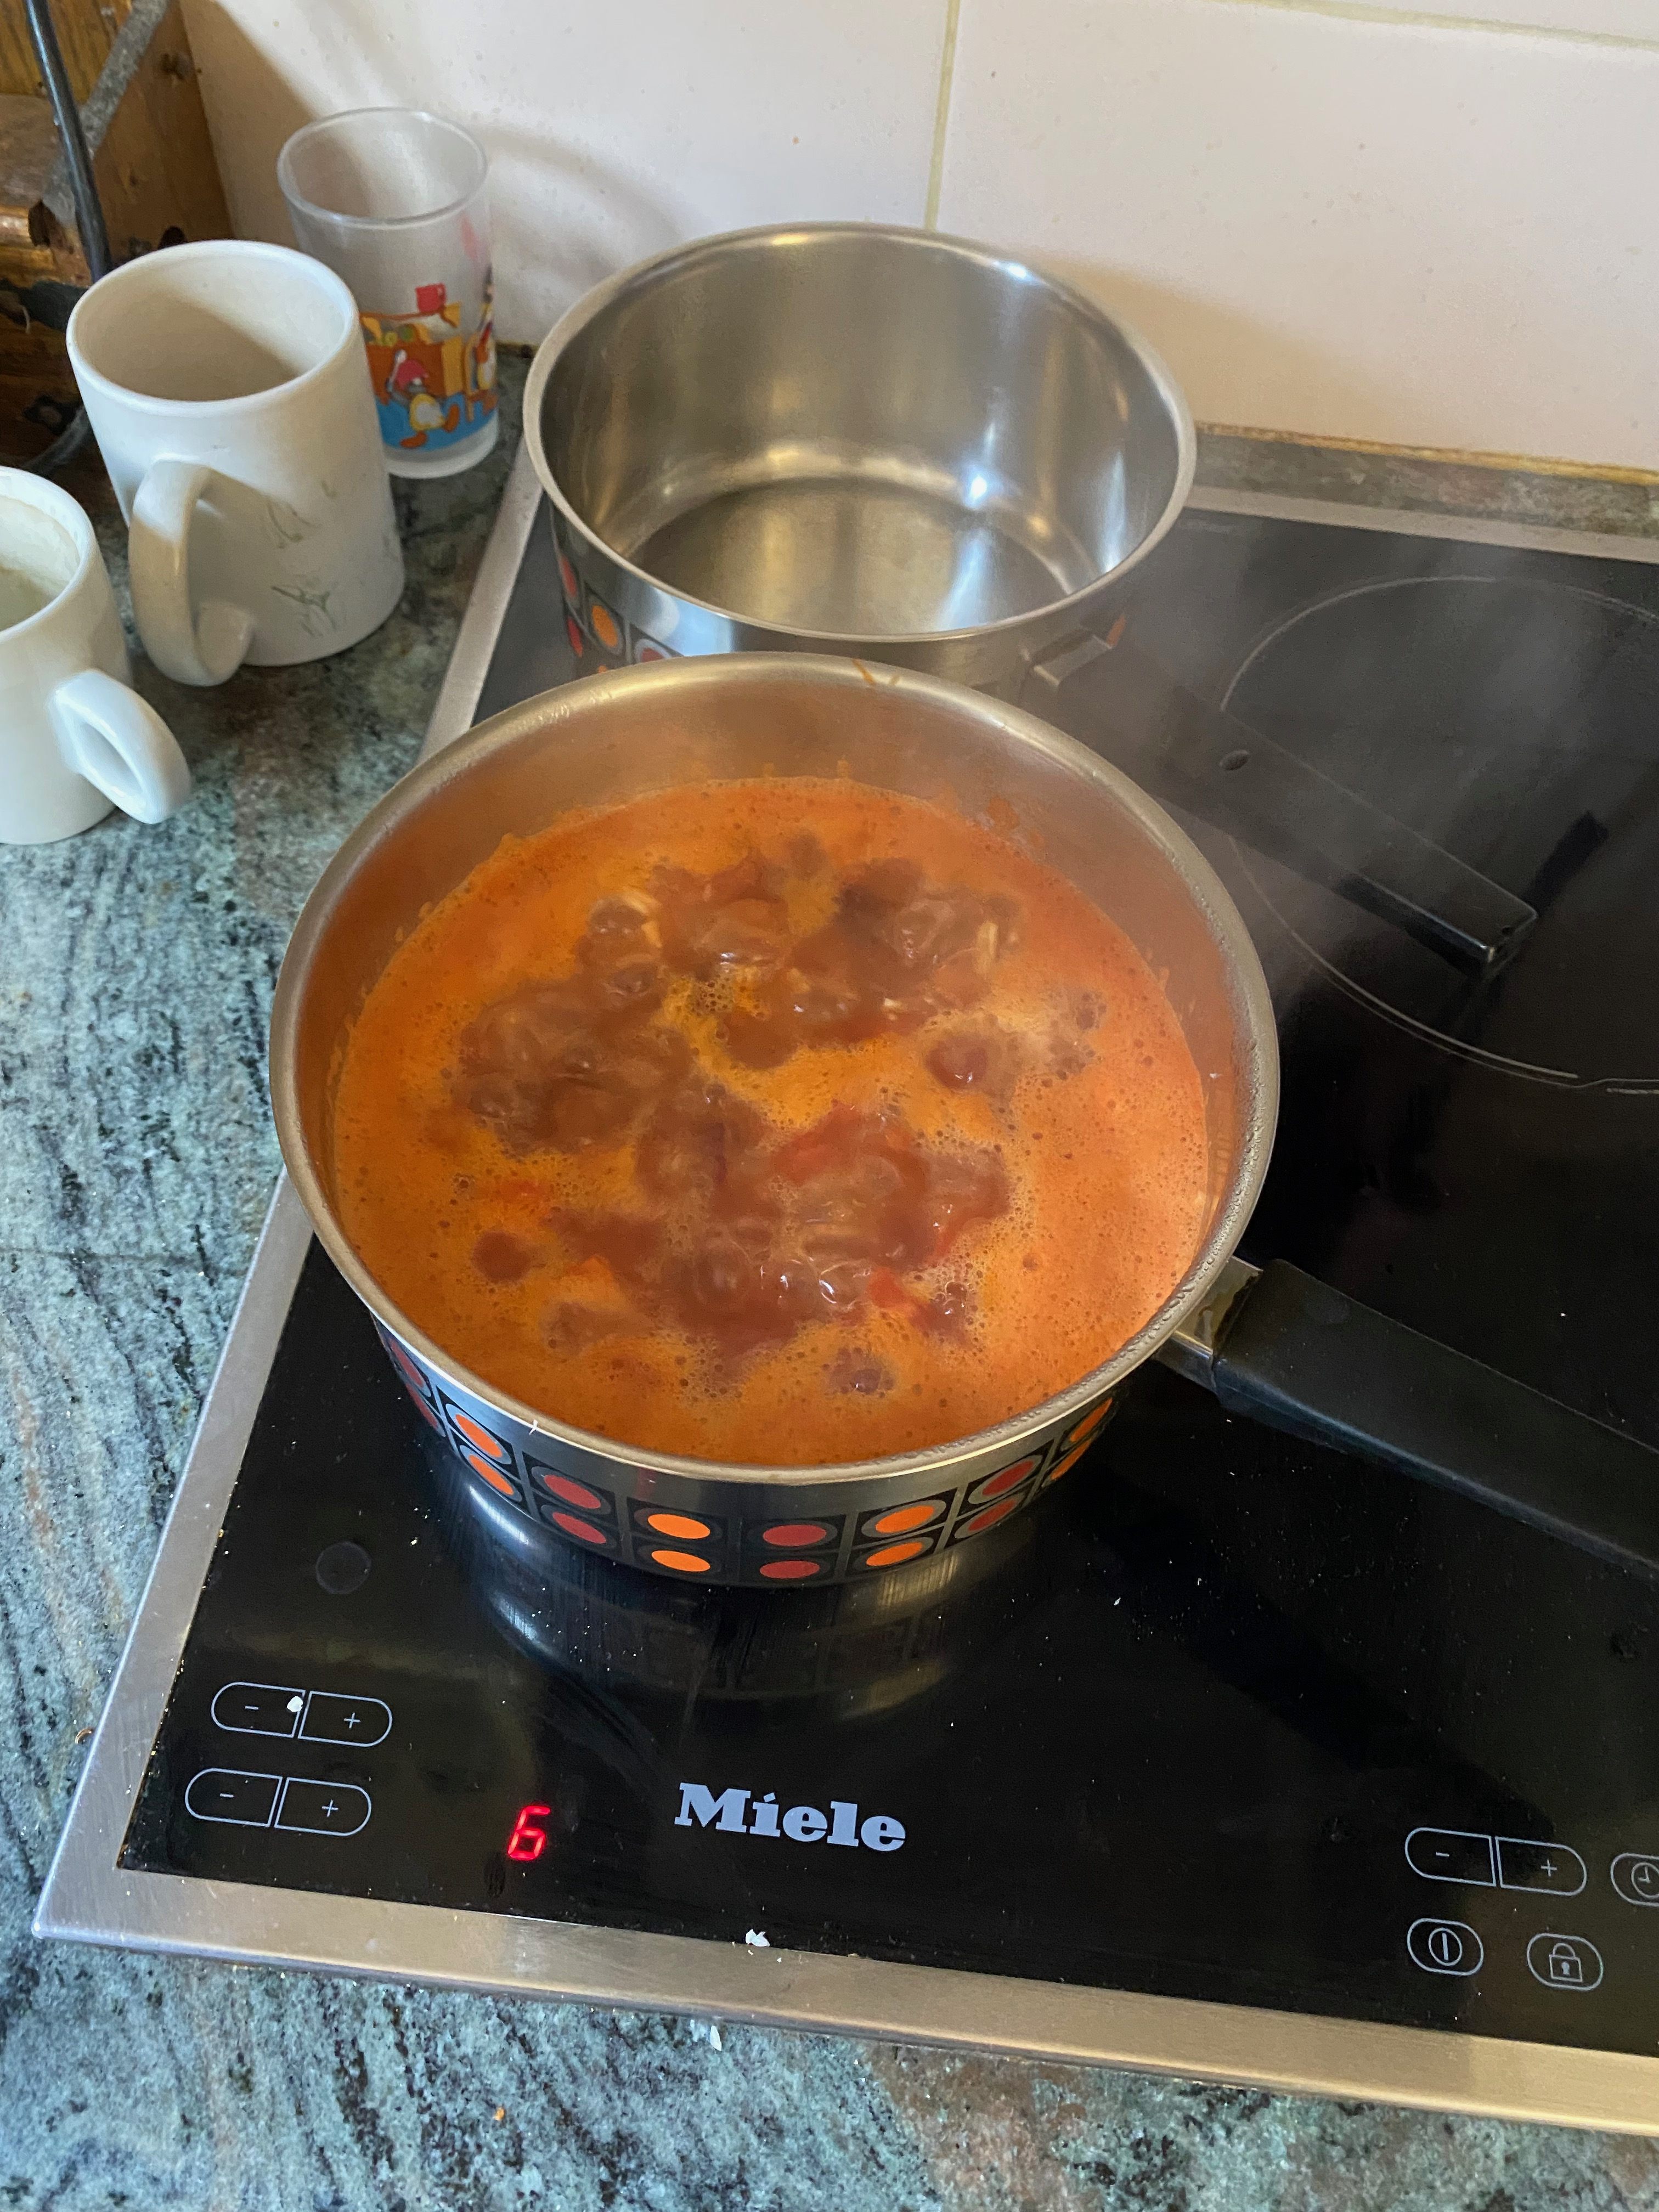
\includegraphics[width=0.48\textwidth]{./assets/curry_de_haricots}}
        \newline
        \newline
        \textbf{Pour 4 personnes}
    \end{multicols}
\end{document}